\documentclass[11pt,a4paper,titlepage]{article}

\usepackage[letterpaper,top=1in, bottom=1in, left=1.5in, right=1in]{geometry}
\usepackage{url}
\usepackage{setspace}
\usepackage{listings,multicol}
\usepackage{authoraftertitle}
\usepackage{graphicx}
\usepackage{array}
\usepackage[table]{xcolor} 
\usepackage[nottoc,numbib]{tocbibind}
\usepackage{tocloft} 
\setlength{\cftsecnumwidth}{1.2cm}
\setlength{\cftsubsecindent}{1.2cm}
\renewcommand{\refname}{Bibliography}
\renewcommand\thesection{\Roman{section}.}
\renewcommand\thesubsection{\Alph{subsection}.}
\renewcommand\thesubsubsection{\arabic{subsubsection}.}

\doublespacing

\title {Mammo: An Application of Convolutional Neural Networks on Breast Cancer Screening}
\author {Sigfreed John S. Angeles}
\date{June 2018}

% allows for separate page section by changing the behavior of \section
\let\stdsection\section
\renewcommand\section{\newpage\stdsection}

\newcommand{\Keywords}[1]{\par\noindent 
{\small{\em Keywords\/}: #1}}

\usepackage{bm}
\newcommand{\+}{\discretionary{\mbox{${\bm\cdot}\mkern-1mu$}}{}{}}

\begin{document}
%\maketitle
\begin{titlepage}

\begin{center}


% Upper part of the page

\textsc{\large University of the Philippines Manila}\\
\textsc{\large College of Arts and Sciences}\\
\textsc{\large Department of Physical Sciences and Mathematics}\\[3.5cm]

% Title
\textsc{\Large \MyTitle}\\[3.5cm]

\textsc{\Large (User Manual)} \\[3.5cm]

A special problem in partial fulfillment\\
of the requirements for the degree of\\
\textbf{Bachelor of Science in Computer Science}


\vfill

% Bottom of the page
Submitted by:\\[1.25cm]
\MyAuthor\\
{\MyDate}
\\[1cm]

\end{center}

\end{titlepage}
\pagenumbering{roman}

\doublespacing

\pagenumbering{roman}
\setcounter{page}{3}
\setcounter{tocdepth}{3}
\newpage

\doublespacing

\section{Mammo Server Installation}
\qquad The Mammo web application requires the following dependencies and specifications:

	\subsection{Python Dependencies}
	\hspace{5mm}\textbf{Anaconda Python 3.5.x} is the recommended python distribution. The required python modules to run the system include:
	
			\begin{enumerate}
				\item{flask}
				\item{pdf-kit}
				\item{flask-sqlalchemy}
			\end{enumerate}
	
	\subsection{Mammo Server Machine}
	\hspace{5mm} The recommended requirements for the server include:
			
			\begin{enumerate}
				\item{2 GHz CPU rate or higher}
				\item{Graphics Processing Unit (GPU) specifically a NVIDIA Graphics Card with 3.0 compute capability or higher}
				\item{8 GB RAM or higher}
				\item{Up to 2 GB of free disk space}
			\end{enumerate}

	\subsection{Mammo Client Machine}
	\hspace{5mm} The client side must have any of the following compatible up-to-date web browsers:
	
			\begin{enumerate}
				\item{Google Chrome}
				\item{Mozilla Firefox}
				\item{Safari}
			\end{enumerate}

\section{Mammo Web Application}
	\subsection{Home Screen}
	\qquad The home page of the system is seen in  figure \ref{fig:mammoHome}. A basic description of what the site is for is present here along with the features it has to offer. Also, a navbar that provides the user access to the site's features is present at all pages of the site.
	
	\begin{figure}[h]
		\centering
	  	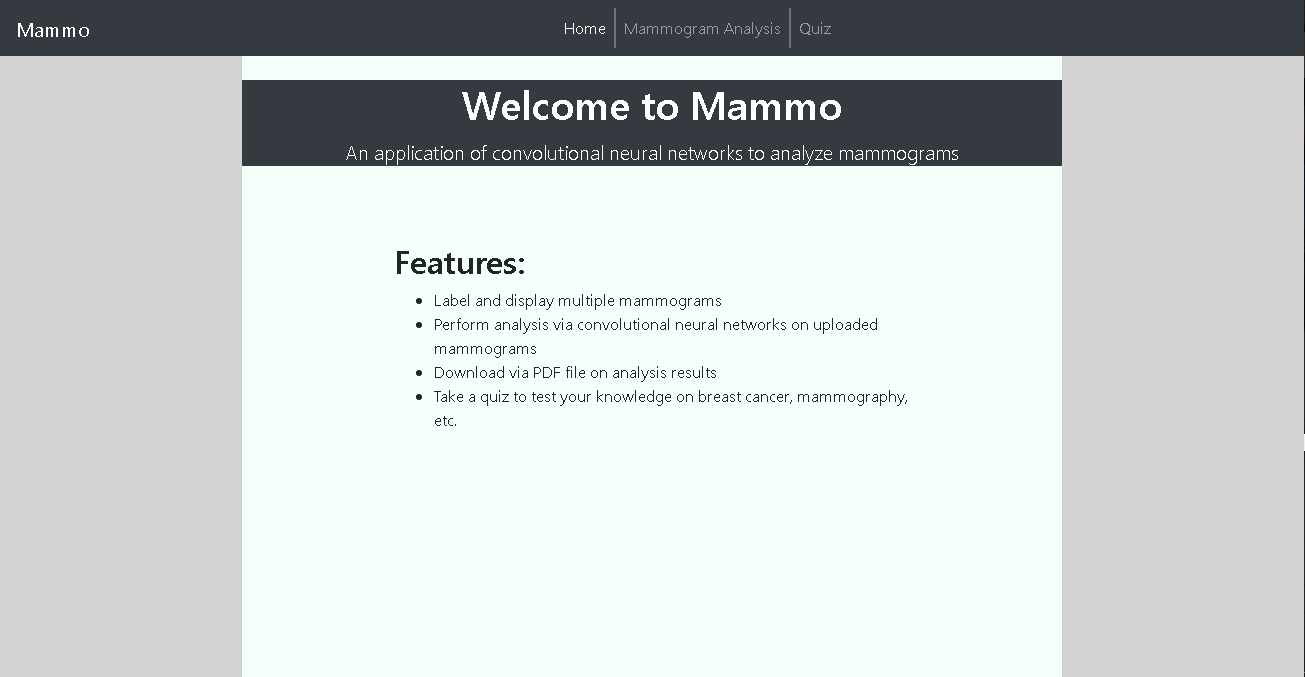
\includegraphics[scale=0.5]{images/mammoHome.png}
		\caption{Mammo home page, Mammo}
	  	\label{fig:mammoHome}
	\end{figure}
	
	\subsection{Mammogram Analysis}
	
	\subsubsection{Uploading Mammograms}
	\qquad Figure \ref{fig:uploadMammograms} shows that a user has fully uploaded his chosen mammograms. A user may do this through the "Add Images" button at the top of the left sidebar or by just dragging and dropping files from his/her directory.
	
	\begin{figure}[h]
		\centering
	  	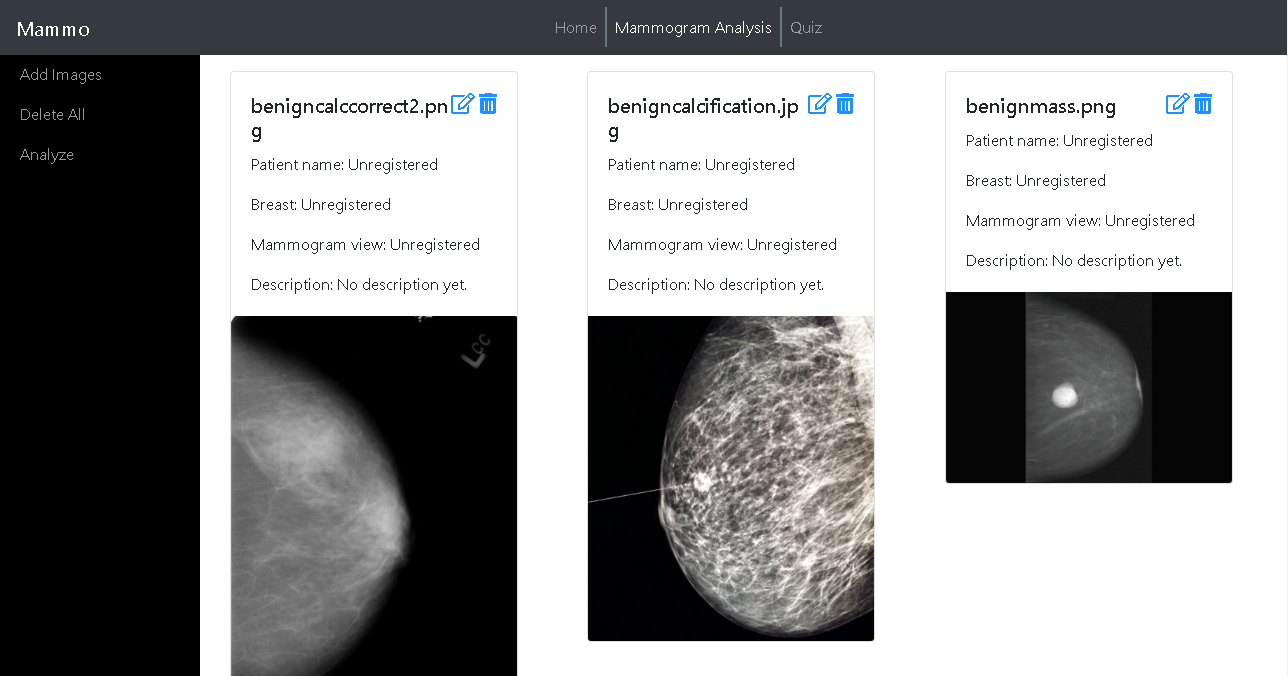
\includegraphics[scale=0.5]{images/uploadMammograms.png}
		 \caption{Three uploaded mammograms, Mammo}
	  	\label{fig:uploadMammograms}
	\end{figure}
	
	\subsubsection{Editing and Deleting Mammograms}
		\qquad The mammograms are uploaded with unregistered metadata that is up for the user to edit. A user may edit the mammograms by clicking the edit icon present at the upper right of the mammogram cards, or he may simple click on the picture of the mammogram as shown figure \ref{fig:editMammograms}. Also, a user may delete the mammogram by pressing the delete icon next to the edit. Moreover, a user may delete all the mammograms uploaded by the "Delete All" button on the sidebar. Also, a user must specify the region of interest to be analyzed by the CNN module. A user may leave the metadata entries blank, but he must choose a region of interest and save it.
	
	\begin{figure}[h]
		\centering
	  	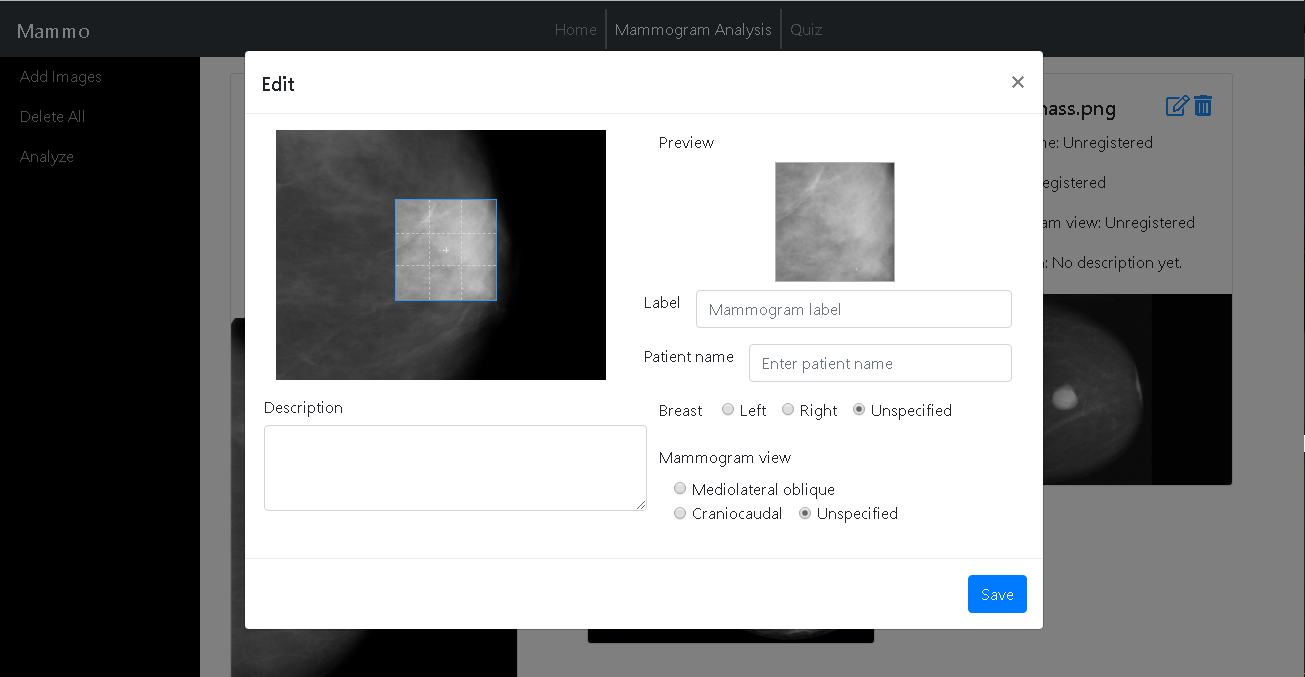
\includegraphics[scale=0.5]{images/editMammograms.png}
		 \caption{Editing metadata of the mammogram, Mammo}
	  	\label{fig:editMammograms}
	\end{figure}
	
	
	\subsubsection{Analyzing the Mammograms}
		\qquad After the user has entered the necessary patient data, he/she may then proceed to have the mammograms analyzed by the "Analyze Mammograms" on the sidebar (see figure \ref{fig:uploadMammograms}). It may take a long time to process the mammograms. Figures \ref{fig:mammogramAnalysis1} and \ref{fig:mammogramAnalysis2} show the analysis made by the CNN module. A "Generate PDF" functionality is present for the user to save the results as PDF (see figure \ref{fig:mammogramPDF}).
	
	\begin{figure}[h]
		\centering
	  	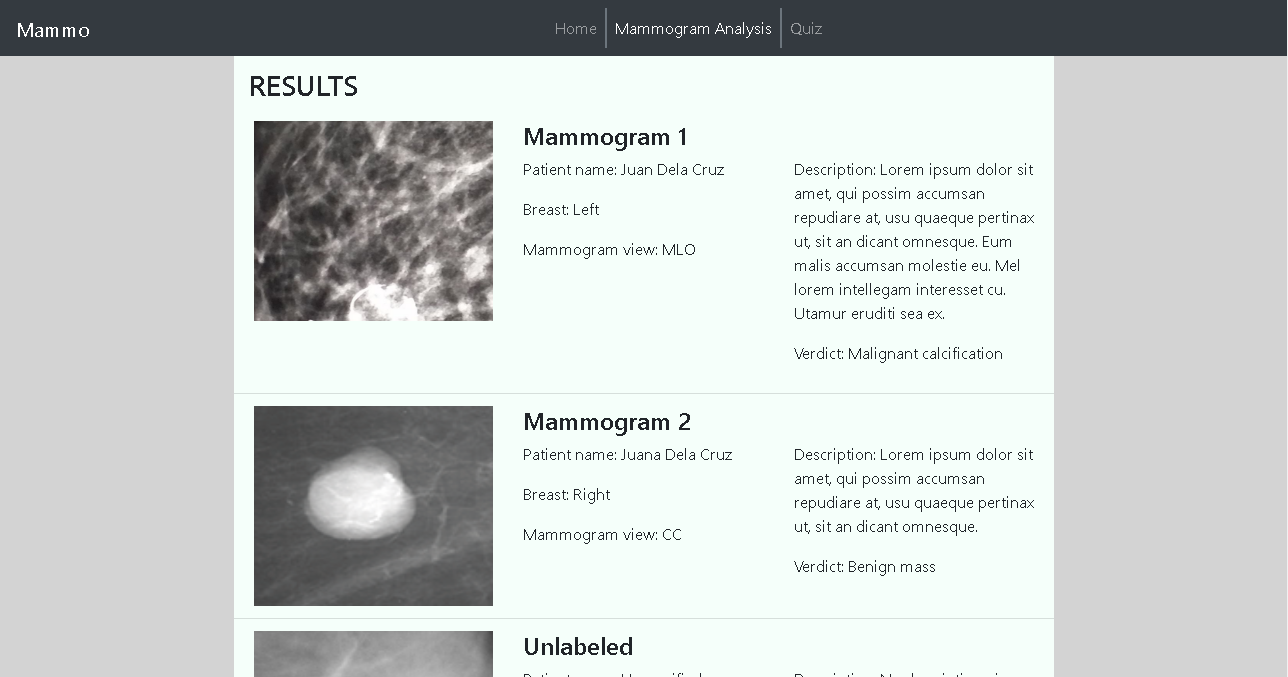
\includegraphics[scale=0.5]{images/mammoAnalysis1.png}
		 \caption{Results of the analysis made by the CNN module part 1, Mammo}
	  	\label{fig:mammogramAnalysis1}
	\end{figure}
	
	\begin{figure}[h]
		\centering
	  	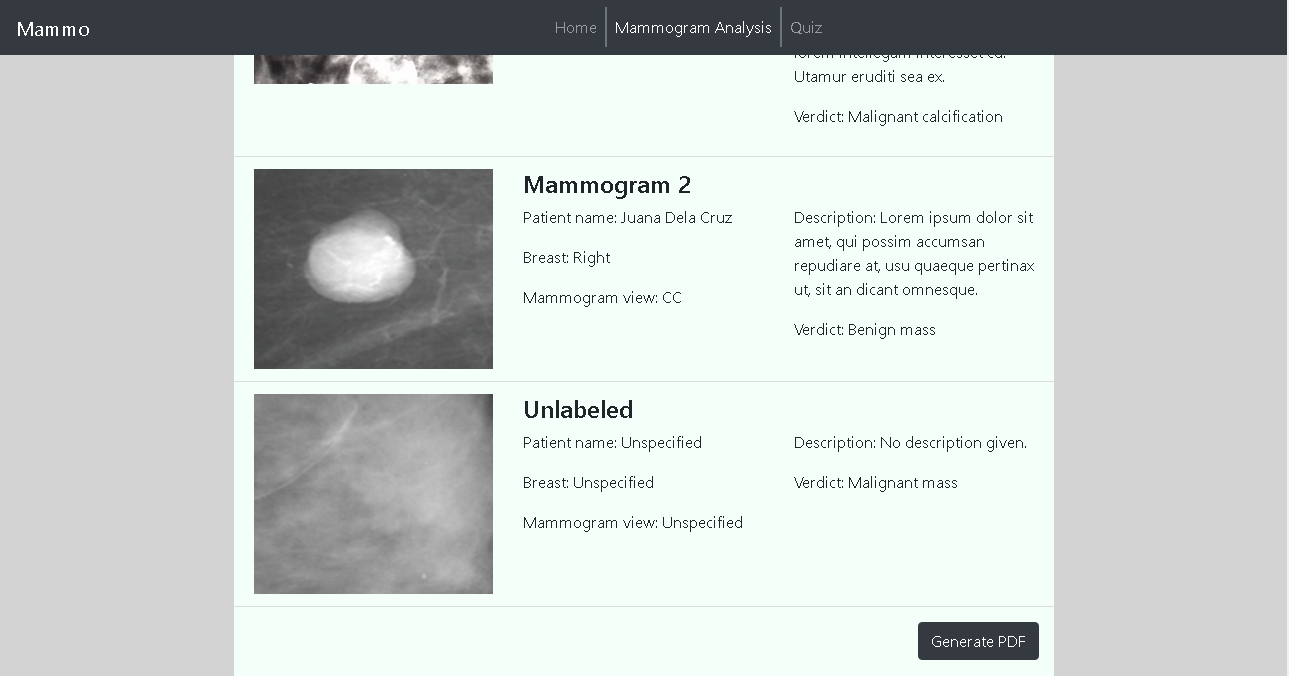
\includegraphics[scale=0.5]{images/mammoAnalysis2.png}
		 \caption{Results of the analysis made by the CNN module part 2, Mammo}
	  	\label{fig:mammogramAnalysis2}
	\end{figure}
	
	\begin{figure}[h]
		\centering
	  	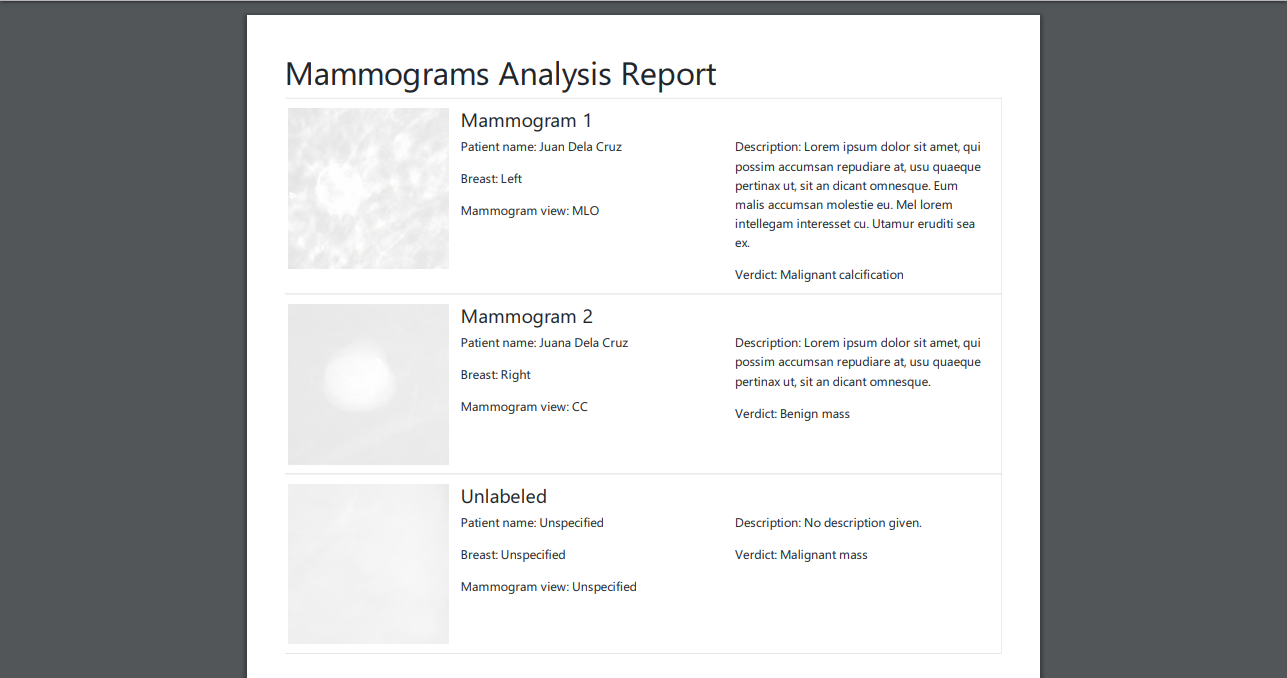
\includegraphics[scale=0.5]{images/mammogramPDF.png}
		 \caption{A generated PDF file of Mammogram Analysis Report, Mammo}
	  	\label{fig:mammogramPDF}
	\end{figure}
	
	\subsection{Quiz}
	
	\subsubsection{Taking the Quiz}
	\qquad A user or a student/trainee has the option to take a randomly-generated 10-item pop quiz regarding breast cancer, mammography, treatment, etc. (see figure \ref{fig:mammogramExam}).
	
	\begin{figure}[h]
		\centering
	  	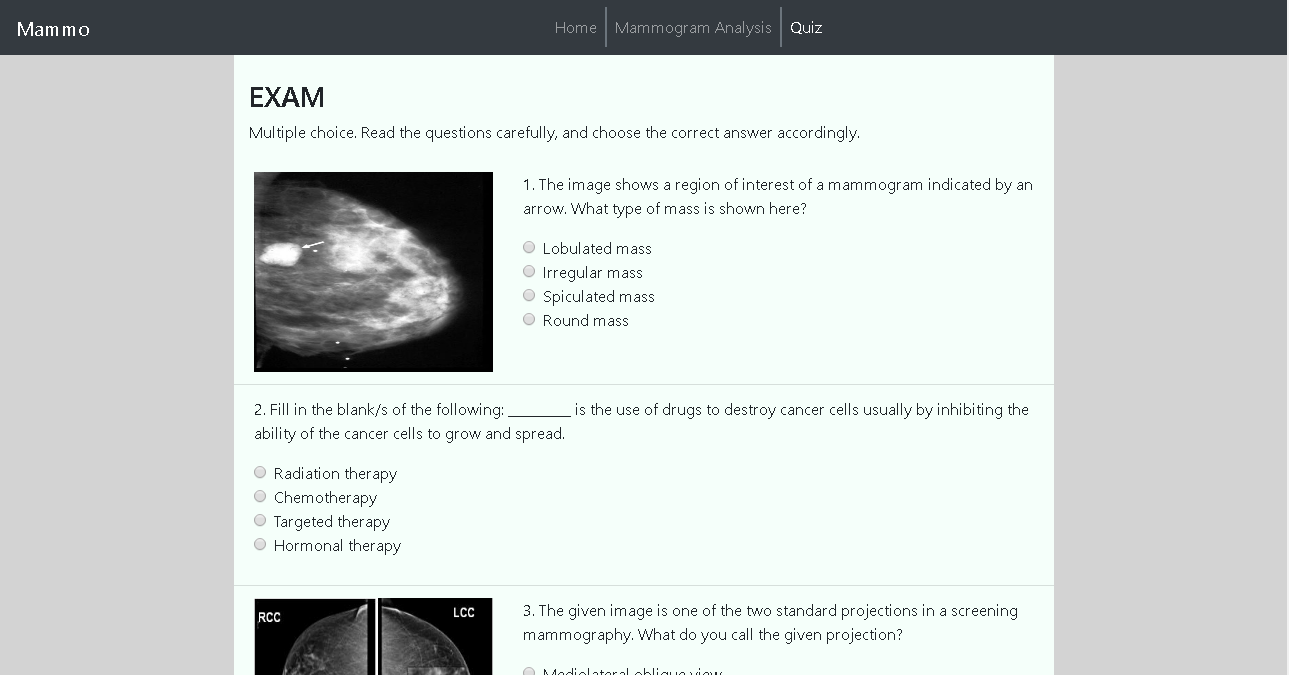
\includegraphics[scale=0.5]{images/mammogramExam.png}
		 \caption{A sample of the quiz, Mammo}
	  	\label{fig:mammogramExam}
	\end{figure}
	
	\subsubsection{Quiz Results}
	\qquad After the user has answered the questions and reviewed the answers, he/she may submit the quiz for evaluation by the "Submit" button seen in figure \ref{fig:submitQuiz}.
	
	\begin{figure}[h]
		\centering
	  	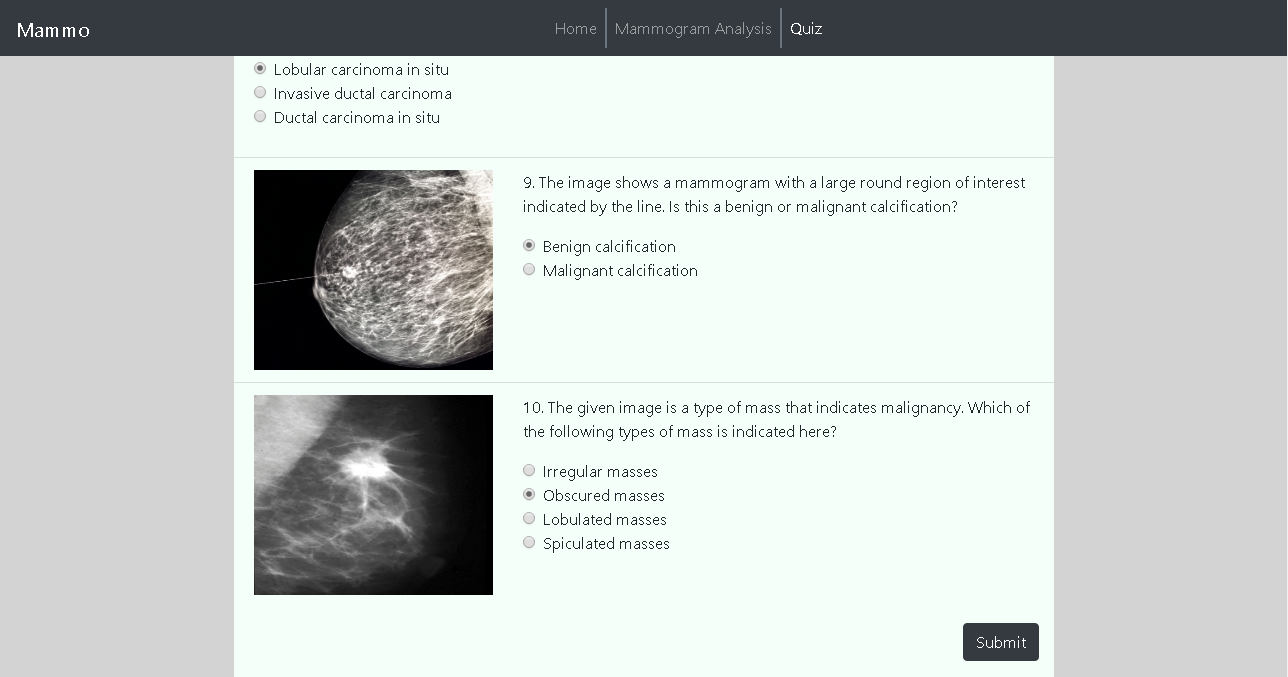
\includegraphics[scale=0.5]{images/submitQuiz.png}
		 \caption{Submit the quiz, Mammo}
	  	\label{fig:submitQuiz}
	\end{figure}
	
		The user's score and the correct answer are seen in figure \ref{fig:quizResults}.
	
	\begin{figure}[h]
		\centering
	  	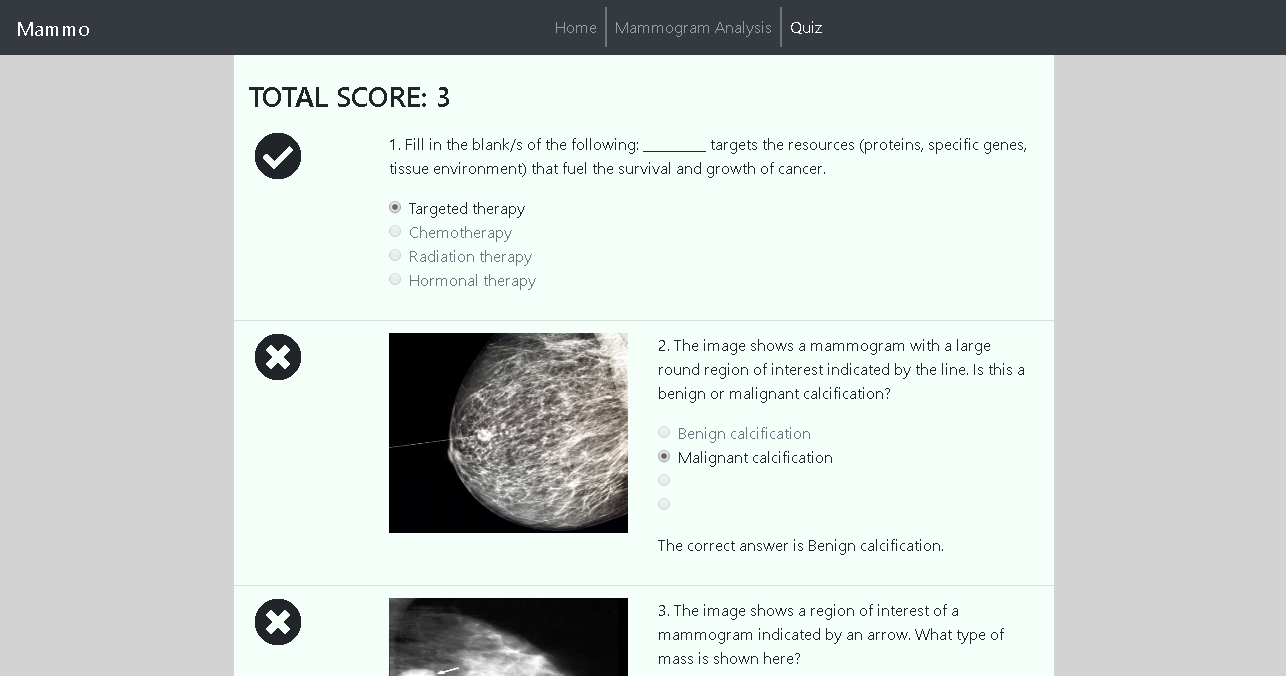
\includegraphics[scale=0.5]{images/quizResults.png}
		 \caption{Results of the quiz, Mammo}
	  	\label{fig:quizResults}
	\end{figure}
\end{document}


